\documentclass{article}
\usepackage[UTF8]{ctex}
\usepackage{geometry}
\usepackage{graphicx} % 插图宏包
\usepackage{float} % 提供H位置参数，让图片固定在想要的位置
\geometry{a4paper, margin=2.5cm}

\begin{document}

\title{我眼中的大气科学：来自七节讲座的专业认知}
\author{姓名：魏金勇\\班级：大气科学类2025级13班\\学号：202583300520}
\date{}
\maketitle

\section{观：我印象最深的一次讲座和它的内容}

在七次大气科学专业基础讲座里面，让我印象最深的那个是第五讲，名字叫《智慧气象：当人工智能遇见天气预报》。讲课的老师是人工智能学院的一个老师，他做的事情是数据同化和数值模式研究，也研究机器学习怎么用在气象里面。

这次讲座分成四个部分。第一个部分讲的是传统天气预报的基本流程，大概就是先采集观测数据，然后做资料同化，再去算数值模式，算完之后做一个后处理订正，最后让预报员来做综合判断。老师说了，这套流程虽然在过去几十年进步非常大，但是计算成本很高，还有一些次网格的物理过程用的参数化方案，本身就有挺大的不确定性 \cite{陈德辉2004数值}。

第二个部分说的是人工智能怎么走进气象领域，主要的路径有这几个：一个是用卷积神经网络去识别台风螺旋雨带和中气旋这些天气系统 \cite{Lecun2015Deep}，另一个是用循环神经网络或者Transformer架构来做雷达回波的外推 \cite{Shi2015Convolutional}，还有一个是用生成对抗网络去搞高分辨率的降尺度 \cite{Reichstein2019Deep}。

第三个部分是讲座的亮点，老师详细讲了华为云做的那个盘古气象大模型 \cite{Bi2022}，这个模型跟传统的数值模式不一样，它是基于三维Transformer架构的，先在再分析资料上做了大规模的预训练，然后在几秒钟里面就能输出全球的中期预报结果。在有些要素上面比如位势高度和温度，它的预报误差比欧洲中期天气预报中心的传统数值模式还要低。

第四个部分讲的是现在AI气象面临的主要挑战，一个是模型不太能被解释清楚，另一个是对极端天气事件的学习能力不太好因为样本太少了，还有一个是怎么把AI跟现有的资料同化系统好好结合起来 \cite{McGovern2019Making}。讲座快要结束的时候，老师展示了一张能耗对比图，传统数值模式预报一次用的电相当于一个普通家庭好几个月的用电量，但是盘古模型在几张GPU卡上面就能把推理做完，这个对比给在场的同学都留下了很深的印象。

\begin{figure}[H]
\centering
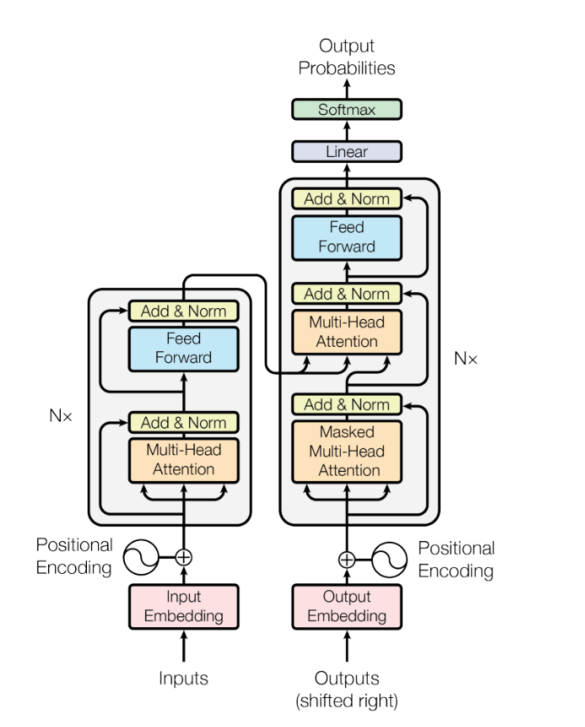
\includegraphics[width=0.7\textwidth]{fig1.png}
\caption{图1：Transformer架构模型示意图}
\end{figure}

\begin{figure}[H]
\centering
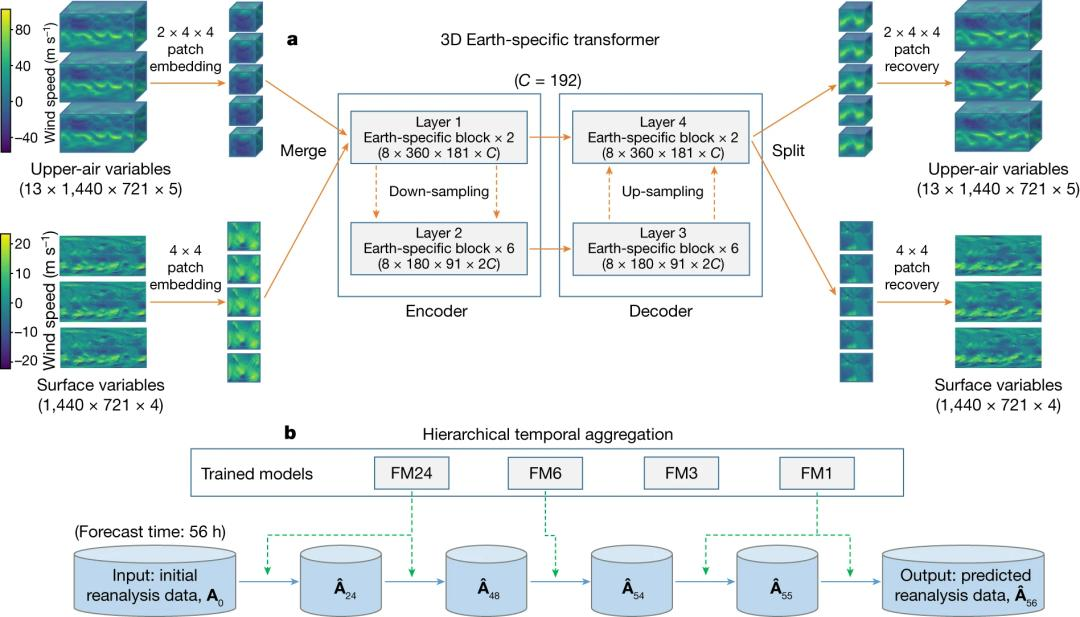
\includegraphics[width=0.7\textwidth]{fig2.jpg}
\caption{图2：盘古气象大模型示意图}
\end{figure}

\section{感：这节讲座为什么让我印象很深}

这节讲座让我印象很深，原因大概有三个。

第一个原因是，这个话题跟我自己的知识背景比较合得来。我高中的时候自己学过Python编程，也接触过一些基础的机器学习概念比如说卷积神经网络和反向传播这些，虽然没有正儿八经的竞赛或者项目经验，但是对计算机和算法一直挺感兴趣的。进了大气科学专业以后有一阵子还挺困惑的，不知道怎么能把这两个兴趣放在一起，这节讲座很清楚地展示了AI和大气科学交叉的那个领域，就是智慧气象或者AI气象学，算是给我指了一个具体而且能走得通的方向。

第二个原因是，这个老师的表达风格很清楚也很实在，他既不躲着技术细节走，也不会故意说一些难懂的话让人觉得有距离感。比如说讲盘古模型的时候他直接就展示了模型的网络结构示意图，还解释了Transformer里面的自注意力机制为什么适合用来处理大气数据，因为大气不同区域之间有长距离的依赖关系。这种把原理讲清楚同时又给一个直观理解的办法，让我在自己专业知识还不太够的情况下也能抓住核心的意思。

第三个原因是，讲座的内容本身有很强的现实冲击力。老师对比传统数值模式和AI模型的计算能耗的时候，我突然意识到AI不仅仅是算得更快的问题，它可能会从根本上改变气象预报的工程范式。一个在单台服务器上就能跑起来的预报系统，意味着发展中国家还有偏远地区甚至个人研究者都有机会拿到过去只有顶级气象中心才能负担得起的预报能力 \cite{Bauer2015Quiet}，这种技术带来的公平性提升我觉得挺有社会意义的。

\section{思：那些引起我兴趣和思考的知识点或者观点}

讲座里面有这么几个观点引起了我的兴趣和思考，有些我课后还专门去查了查资料。

第一个是AI能不能代替数值模式里面的物理参数化方案这个问题 \cite{Schneider2017Earth}。传统的数值模式里面次网格的过程比如说积云对流和边界层湍流，必须用参数化方案来做一个近似的表达，而这些方案本身就带了很多经验性的假设。老师说有研究在尝试用神经网络直接去学次网格通量和网格尺度变量之间的映射关系，然后代替传统的参数化方案 \cite{Brenowitz2018Prognostic}。这让我想到两个层面的东西，一个方面是纯靠数据驱动的参数化方案会不会违背基本的物理守恒律，另一个方面是如果训练数据是从高分辨率的云解析模式里面输出的，那么AI学到的那个物理其实只是另一种数值近似而不是真实的大气过程。这个问题好像不是那么容易回答的。

第二个是极端天气的小样本学习问题 \cite{Gagne2014Machine}。讲座里面说到对于台风、龙卷、极端暴雨这些比较稀有的天气事件，能用来训练的历史样本特别少，这就导致AI模型遇到极端情况的时候往往表现不太好。老师上课的时候举了个例子说有一个AI模型做常规降水预报的时候表现挺好的，但是有一次碰到百年一遇的暴雨事件，预报出来的结果就明显偏低了。这让我想起来机器学习里面常说的分布外泛化问题，就是训练集和测试集的分布不一样的时候，模型的性能会掉得很厉害。怎么让AI学会去应对没见过的情况，可能需要引入物理约束或者数据增强或者元学习这些方法，这个方向我觉得挺有挑战性的，也挺有研究价值的。

第三个是AI预报的不可解释性问题 \cite{Ham2020Deep}。传统的数值模式虽然复杂，但是每一步都是根据物理方程来的，预报员可以追着误差去找它的来源。可是深度学习的黑箱特性让预报员很难搞明白一个AI预报结论背后的依据是什么。老师说现在的趋势是去做可解释AI，比如说通过注意力图或者特征可视化来告诉预报员模型关注了哪些地方 \cite{Tjoa2020Survey}。但是这类方法是不是真的能提供靠谱的物理解释，现在还是有争议的。我自己觉得如果AI要成为预报决策里头一个可信的工具，而不是只提供一个参考的黑箱，那可解释性就一定要从根本上解决掉。

\section{探：对某一个具体研究方向的调研和理解}

因为上面的那些思考，我就选了人工智能气象这个方向去做了一点更细的调研，下面是我查了一些资料以后形成的对这个方向的理解。

\subsection{主要研究什么}

AI气象学的研究范围还挺广的，现在比较活跃的小方向有这几个。

第一个是雷达回波的外推和短时临近预报，用的是循环神经网络或者卷积LSTM或者基于注意力机制的模型，根据过去几个时刻的雷达反射率因子图像去预测未来零到六小时的雷达回波会怎么变 \cite{Shi2015Convolutional}。跟传统的光流法比起来，深度学习方法能更好地抓住对流单体的生消、合并和分裂这些非线性的过程。

第二个是数值预报的AI后处理，传统的后处理方法有模式输出统计和集合订正这些。最近几年研究者开始用随机森林或者梯度提升或者小型的神经网络来对数值模式的输出做偏差订正和概率化预报 \cite{Rasp2018Deep}，这样能明显提高降水和风速这些要素的预报精度。

第三个是气象大模型，盘古气象 \cite{Bi2022}、GraphCast \cite{Lam2023}、FourCastNet \cite{Pathak2022FourCastNet} 这些都算，这类模型直接在大型的再分析资料集上面做预训练，用的是Transformer或者图神经网络的结构，做到了跟传统数值模式差不多甚至更好的中期预报效果。好处是计算效率特别高，不好的地方是很难把实时的观测数据融进去，目前还是以后处理的方式在用。

第四个是物理引导的机器学习 \cite{Kashinath2021Physics}，为了不让纯数据驱动的模型违反物理规律，研究者试着把控制方程比如说纳维斯托克斯方程当成一个约束项或者损失函数嵌到神经网络的训练过程里面去。这种方法在保持计算效率的同时还能维持一定的物理一致性。

\subsection{社会意义}

AI气象的社会意义可以从两个层面来看。从防灾减灾的层面来说，更快的预报速度和更高的准确性意味着能更早发出预警也能准备得更充分。比如说如果能把这个强对流的预警提前量从现在的二十到四十分钟提升到六十分钟以上，人员伤亡和财产损失应该都能少不少。从普惠服务的层面来说，AI模型比较低的计算成本让高质量的预报不再只能靠有超级计算机的发达国家才能做 \cite{世界气象组织2021智慧}。对于非洲、东南亚这些气象观测和计算资源相对比较少的地方来说，这个现实意义挺大的。

\subsection{发展前景}

从现在的发展趋势来看，未来五到十年AI气象很可能会形成一个混合范式，就是数值模式负责给出物理一致的背景场，AI模块负责快速生成特定要素的精细预报或者对数值模式的输出做智能订正。同时端到端的纯AI预报模型也会继续往前走，但是短期之内很难完全取代数值模式，特别是在极端事件和长期气候预测这些领域里面 \cite{Schultz2021Can}.

我自己觉得可解释性、还有不确定性量化、还有实时数据同化，会是AI气象下一阶段需要重点去突破的三个瓶颈。把这些东西解决了，AI气象才能真正从实验室里的玩具变成业务上能用的工具。

\begin{figure}[H]
\centering
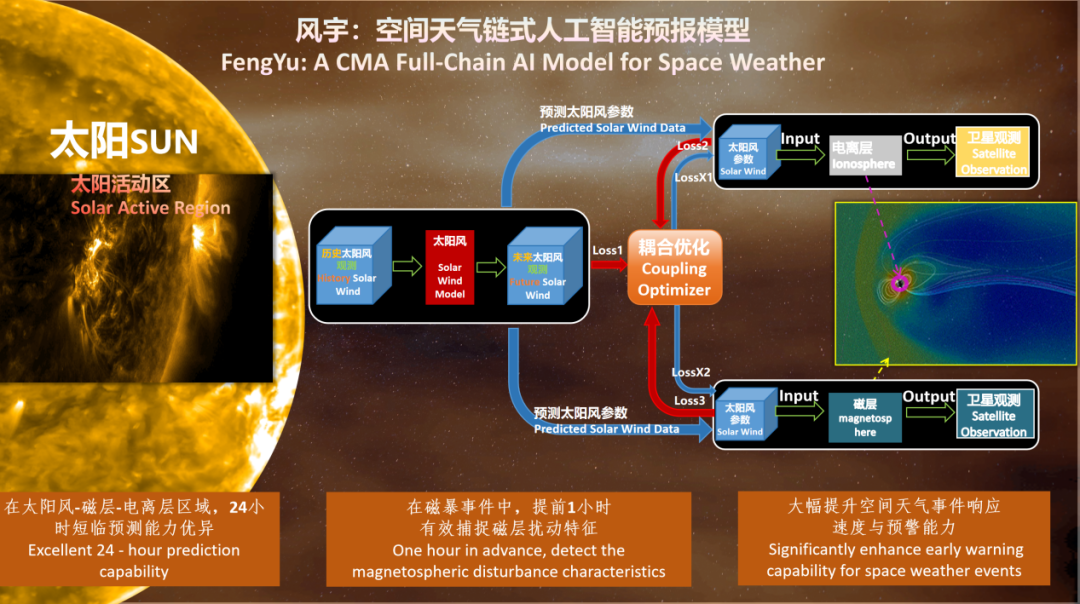
\includegraphics[width=0.4\textwidth]{fig3.png}
\caption{图3：风宇模型示意图}
\end{figure}
\begin{figure}[H]
\centering
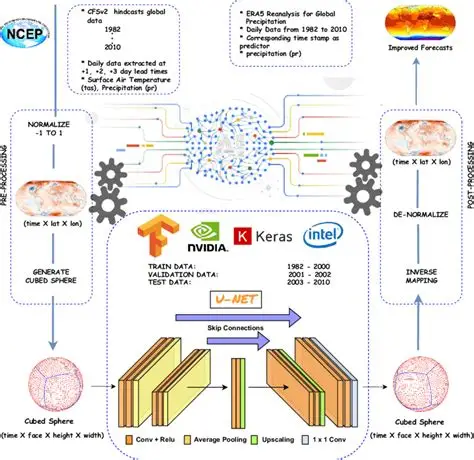
\includegraphics[width=0.4\textwidth]{fig4.png}
\caption{图4：NCEP示意图}
\end{figure}

\section{择：我对这个方向的兴趣和将来可能会做的选择}

听了这个课又自己去查了一些东西之后，我对人工智能气象这个交叉方向有了比较明确的兴趣，也初步把它当成未来专业发展的一个可能的方向。

兴趣的来源有两个地方。一个地方是它正好落在我现有的知识储备和以后要学的目标之间。我有一点编程基础也一直对机器学习挺有兴趣的，大气科学专业的课又在慢慢帮我把天气气候的物理机制给搭起来。AI气象要求这两方面的素养都得有，这让我觉得我不是从零开始而是站在一个还算有利的起点上面。另一个地方是这个方向既有理论的深度又有实际的应用价值。大气系统的非线性、多尺度和混沌特性给机器学习研究提供了一个挺有挑战性的应用场景，同时AI气象的成果可以直接变成防灾减灾的效益，这种学完了能用来做事的感觉是我比较看重的。

关于以后的规划，我现在的想法是这样的。本科阶段我需要同时把三个方面的基础给加强一下。一个是大气的核心课程特别是动力气象、天气学、雷达气象和云物理学，一个是数学和统计的基础比如说概率论、数理统计和时间序列分析，还有一个是计算机和数据科学的技能像Python编程、PyTorch或者TensorFlow框架还有基础的机器学习算法。我打算在大二或者大三的时候试着进学院里面做AI气象研究的课题组，去参与一些比较简单的科研训练项目，比如说搭一个小型的雷达回波外推模型，或者帮着做一做气象数据集的清洗和标注。这些经历能帮我更具体地判断自己是不是真的适合做这个方向。

毕业以后的选择我现在偏向于继续读研究生，去深入研究AI气象里面的某一个具体的问题，比如极端天气的小样本学习或者物理约束的神经网络或者AI在资料同化里面的应用这些 \cite{Geer2020Machine}。最终的目标是能进到气象的业务部门或者研究机构里面，去做AI气象模型的研发和业务化应用的工作。

我也很清楚这个方向现在还有很多没有解决的问题，可解释性、泛化能力和物理一致性这些都在那儿摆着。但是恰恰是这些挑战让研究变得有价值，一个有困难但是还在成长的领域，可能刚好适合愿意同时面对物理和代码的人。

\begin{thebibliography}{99}

\bibitem{陈德辉2004数值}
陈德辉, 薛纪善. 数值天气预报业务模式现状与展望[J]. 气象学报, 2004, 62(5): 623-633.

\bibitem{Lecun2015Deep}
LeCun Y., Bengio Y., Hinton G. Deep learning[J]. Nature, 2015, 521(7553): 436-444.

\bibitem{Shi2015Convolutional}
Shi X., Chen Z., Wang H., et al. Convolutional LSTM network: A machine learning approach for precipitation nowcasting[C]. Advances in Neural Information Processing Systems, 2015: 802-810.

\bibitem{Reichstein2019Deep}
Reichstein M., Camps-Valls G., Stevens B., et al. Deep learning and process understanding for data-driven Earth system science[J]. Nature, 2019, 566(7743): 195-204.

\bibitem{Bi2022}
Bi K., Xie L., Zhang H., et al. Pangu-Weather: A 3D high-resolution model for fast and accurate global weather forecast[J]. arXiv preprint arXiv:2211.02556, 2022.

\bibitem{McGovern2019Making}
McGovern A., Lagerquist R., Gagne D.J., et al. Making the black box more transparent: Understanding the physical implications of machine learning[J]. Bulletin of the American Meteorological Society, 2019, 100(11): 2175-2199.

\bibitem{Bauer2015Quiet}
Bauer P., Thorpe A., Brunet G. The quiet revolution of numerical weather prediction[J]. Nature, 2015, 525(7567): 47-55.

\bibitem{Schneider2017Earth}
Schneider T., Lan S., Stuart A., et al. Earth system modeling 2.0: A blueprint for models that learn from observations and targeted high-resolution simulations[J]. Geophysical Research Letters, 2017, 44(24): 12396-12417.

\bibitem{Brenowitz2018Prognostic}
Brenowitz N.D., Bretherton C.S. Prognostic validation of a neural network unified physics parameterization[J]. Geophysical Research Letters, 2018, 45(12): 6289-6298.

\bibitem{Gagne2014Machine}
Gagne D.J., McGovern A., Xue M. Machine learning enhancement of storm-scale ensemble probabilistic quantitative precipitation forecasts[C]. 27th Conference on Severe Local Storms, 2014.

\bibitem{Ham2020Deep}
Ham Y.G., Kim J.H., Luo J.J. Deep learning for multi-year ENSO forecasts[J]. Nature, 2020, 573(7775): 568-572.

\bibitem{Tjoa2020Survey}
Tjoa E., Guan C. A survey on explainable artificial intelligence (XAI): Toward medical XAI[J]. IEEE Transactions on Neural Networks and Learning Systems, 2020, 32(11): 4793-4813.

\bibitem{Rasp2018Deep}
Rasp S., Leroux S. Deep learning for post-processing ensemble weather forecasts[J]. arXiv preprint arXiv:1805.09091, 2018.

\bibitem{Lam2023}
Lam R., Sanchez-Gonzalez A., Willson M., et al. GraphCast: Learning skillful medium-range global weather forecasting[J]. Science, 2023, 382(6677): 1416-1421.

\bibitem{Pathak2022FourCastNet}
Pathak J., Subramanian S., Harrington P., et al. FourCastNet: A global data-driven high-resolution weather model using adaptive Fourier neural operators[J]. arXiv preprint arXiv:2202.11214, 2022.

\bibitem{Kashinath2021Physics}
Kashinath K., Mustafa M., Albert A., et al. Physics-aware machine learning for Earth science[J]. AGU Fall Meeting Abstracts, 2021.

\bibitem{Schultz2021Can}
Schultz M.G., Betancourt C., Gong B., et al. Can deep learning beat numerical weather prediction?[J]. Philosophical Transactions of the Royal Society A, 2021, 379(2194): 20200097.

\bibitem{世界气象组织2021智慧}
世界气象组织(WMO). 智慧气象与人工智能应用报告[R]. 日内瓦: WMO, 2021.

\bibitem{Geer2020Machine}
Geer A.J. Learning earth system models from observations: machine learning for data assimilation[J]. ECMWF Technical Memorandum, 2020, 876.

\end{thebibliography}

\end{document}
